\section{\system Overview}\label{sec:overview}
\begin{figure*}
    \centering
    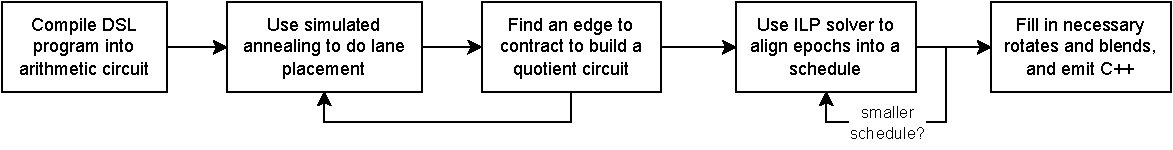
\includegraphics[width=0.8\linewidth]{figures/coyote_algorithm_overview.drawio.pdf}
    \caption{High-level compilation steps}\label{fig:high-level-compilation-steps}
    \Description{Flowchart describing the steps to Coyote's compilation algorithm}
\end{figure*}
\system provides an embedded DSL (eDSL) that allows programmers to use a high level language to express computations in FHE. This computation is translated into an arithmetic circuit representing the computation, which is then compiled into vectorized FHE code. The process of compiling a circuit into vectorized code is as follows: %\milind{overview figure?}

% \milind{You should put the step-by-step procedure for coyote here, then describe them in more detail: break the computation down into aligned subgraphs, assigning scheduling slots, choosing lanes. This is also a good place for a picture explaining these steps: show a tree, show picking bits of a tree, show moving when the computations happen around, show lane assignment}

% \milind{This whole section will benefit from having a running example :-)}
 
\subsection{Compilation Steps}
\begin{figure}
    \begin{subfigure}{0.45\columnwidth}
        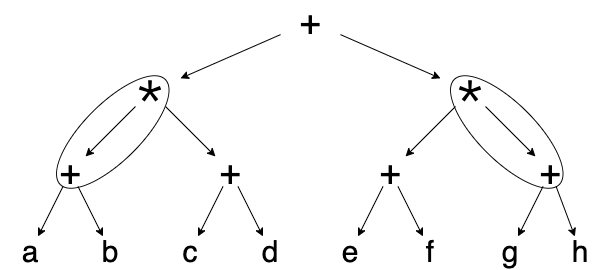
\includegraphics[width=0.9\linewidth]{figures/compilation_overview/running_example_quotiented.drawio.png}
        \caption{Circuit with subcircuits identified}
        \label{fig:subcircuits-identified}
    \end{subfigure}
    \begin{subfigure}{0.45\columnwidth}
        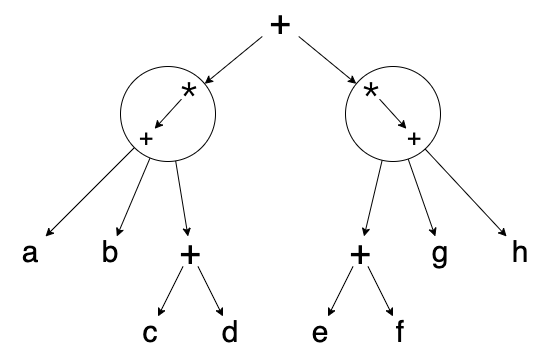
\includegraphics[width=0.9\linewidth]{figures/compilation_overview/running_example_identified.drawio.png}
        \caption{Quotiented circuit}
        \label{fig:quotiented-circuit}
    \end{subfigure}
    \begin{subfigure}{0.55\columnwidth}
        \centering
        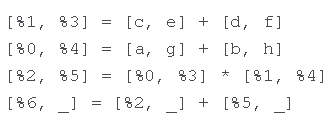
\includegraphics[width=0.9\linewidth]{figures/compilation_overview/aligned_schedule.drawio.pdf}
        \vspace{-1em}
        \caption{Vector schedule after alignment}
        \label{fig:aligned-schedule}
    \end{subfigure}
    \begin{subfigure}{0.4\columnwidth}
        \centering
        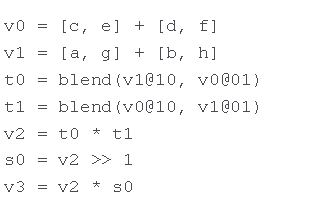
\includegraphics[width=0.9\linewidth]{figures/compilation_overview/generated_vector_ir.drawio.pdf}
        \vspace{-1em}
        \caption{Generated vector code}
        \label{fig:generated-code}
    \end{subfigure}
    \caption{A running example of how \system vectorizes arbitrary arithmetic circuits}
    \label{fig:toy-running-example}
    \Description{Samples of generated code using no vectorization, overly aggressive vectorization, and the optimal vectorization.}
\end{figure}

This section gives an overview of how \system vectorizes an arbitrary arithmetic circuit using the process laid out in Figure~\ref{fig:high-level-compilation-steps}.
We will use the circuit in Figure~\ref{fig:example-circuit} as a running example.
Compilation proceeds as follows:
\begin{enumerate}
    \item \system \textit{quotients} an input circuit (collapses subcircuits into single vertices) and assigns lanes to resulting vertices to produce a {\em pre-schedule} that can be realized into a more efficient vector program. The result is a graph whose vertices correspond to connected subgraphs of the original circuit, such that no two vertices at the same height have the same lane (and hence are eligible to be vectorized together). \system collapses a subcircuit when it determines that the overhead of internally vectorizing it is not worth the gain from vectorization, so this step essentially forces certain operations to happen in scalar on a single lane. %\raghav{I feel I haven't done a good enough job of justifying this.}
    Section~\ref{sec:schedule-search} describes how \system makes this decision. 
    
    In the example in Figure~\ref{fig:subcircuits-identified}, the circled pairs of vertices are collapsed, yielding the quotient circuit in Figure~\ref{fig:quotiented-circuit}.
    The lane assignment for this pre-schedule puts each un-quotiented addition on the same lane as its quotiented parent, and chooses one of these lanes on which to place the root of the tree.
%     \raghav{better?}\milind{This is confusing. Does ``bottom level addition'' mean the addition {\em inside} the subcircuit? Or the other addition that isn't quotiented? I think you need to be more explicit about which operations you're talking about here.} Note that this lane assignment is not intended to be optimal (hence, is a pre-schedule).\raghav{what does this last part mean?}
    
%    \raghav{where do I put this?}
    
    \item The (collapsed) vertices at each height are aligned to pack together isomorphic nodes, producing a vector schedule from the pre-schedule. 
    In the example, the two adds at height 1 get trivially aligned, and the two ``supernodes'' at height 2 get aligned by packing together the two adds and the two multiplies.
    % Since there is a single vertex at height 3, no alignment needs to be done there. 
    No alignment is needed for the single vertex at height 3.
%    \raghav{Is this description clear?}
    The details of the alignment procedure are given in Section~\ref{sec:instruction-alignment}.
    Figure~\ref{fig:aligned-schedule} shows the result of this alignment.
    
    \item \system compiles the schedule into a vector IR. The crux of this compilation step is figuring out when to {\em blend} and {\em rotate}. When a vector operand requires values from several different instructions, \system emits code to ``blend'' the results together into a single vector.
    When the lane an operand is used in is different from the lane it was produced in, \system emits a rotation instruction to move the operand into the correct lane. Notice that each arc in the pre-schedule connecting vertices of different lanes corresponds to a rotation in the generated vector IR.
    Figure~\ref{fig:generated-code} shows the vector code \system generates for our running example.
    Notice that the generated code contains two blends and one rotate.
    The blends are necessary\footnote{In this particular example, exchanging the positions of {\sf \%3} and {\sf \%4} would have produced semantically equivalent code that does not require the blends. However, automatically performing arithmetic rewrites such as this one is outside the scope of this work.} because on line 3 of the schedule, {\sf \%0} and {\sf \%3} are used in the same vector despite being produced in two separate vectors. 
    Since none of the operands need to shift lanes, the vector instruction {\sf t0 = blend(v0@10, v1@01)} takes {\sf [\%0, \%4]} and {\sf [\%1, \%3]} and blends them together to produce {\sf [\%0, \%3]}, which is exactly the operand used on line 3. 
    \system emits a rotation because {\sf \%5} gets used on a different lane than it is produced.
    The vector instruction {\sf s0 = v2 $\gg$ 1} takes {\sf [\%2, \%5]} in {\sf v2} and produces {\sf [\%5, \%2]} in {\sf s0}.
    Section~\ref{sec:codegen} describes the specifics of code generation.
\end{enumerate}
% \raghav{TODO: maybe change the inline texttt stuff so it looks better?}\milind{I tend to prefer {\em {\sf sans serif}} for typesetting inline code, even though it's not monospace}

% \begin{enumerate}
%     \item \system first identifies highly vectorizable subcircuits (shown highlighted in Figure~\ref{fig:small-expr-circuit})
%     \item These subcircuits are pulled out and aligned to produce a single vectorized computation, which is then inserted back into the original program, resulting in the circuit in Figure~\ref{fig:partially-vectorized-circuit}.
%     The challenge with this is aligning the subcircuits optimally; i.e., figuring out which computations can be grouped together into vector operations.
%     Doing this once effectively replaces several subcircuits of the program with a single vectorized circuit, so the process is repeated until no more subcircuits can be found.
%     Each vectorized circuit creates an {\em epoch}, as seen in Figure~\ref{fig:code-split-epochs}.
%     Since the outputs of one epoch are consumed by subsequent epochs, we need to place the outputs in appropriate spots to ensure that the dependences line up.
%     \item The new circuit is converted to a vector {\em schedule} (Figure~\ref{fig:vector-sched-needing-rotates}), which amounts to assigning a {\em lane} (horizontal position) and {\em schedule slot} (vertical position) to each original scalar instruction.
%     \item \system compiles the vector schedule into a vector IR. The crux of this compilation step is figuring out when to {\em blend} and {\em rotate}. When a particular vector operand requires values from several other previously produced vectors, \system emits code to ``blend'' these together into a single vector which can then be used.
    
%     To see why rotates are necessary, notice that in the example schedule, the scalar \texttt{\%3} is computed on lane 2, but used in lane 1. 
%     To correct this discrepancy, \system emits an additional instruction to create a copy of the \texttt{[\%1, \%3]} vector with data arranged as \texttt{[\%3, \%1]}, putting \texttt{\%3} on lane 1 where it is used. %\raghav{Does this flow better?}\milind{yup}
%     % \raghav{Should (3) and (4) go together? Technically (4) is codegen which to me seems like a separate phase of compilation}\milind{It is, but it flows weird -- it's basically a consequence of lane assignment... Or at the very least, write this as a general codegen step, with reference to this example. Right now, it reads as ``this is one specific thing we do'' rather than ``inserting rotation instructions is how codegen works.''}
% \end{enumerate}

% enumerate
% add figure
% \milind{This dives in too quickly; I think the overview thing I laid out above is necessary. Otherwise: what's a stage? What does it mean to schedule subgraphs together? What does it mean to ``line operands up.''}
% \raghav{Is this better? I kind of briefly mentioned ``creating a vector schedule'' as a separate thing that needs to happen apart from just picking vectorizable trees, should I say any more or less about that here, before discussing it in detail in Section~\ref{sec:design}?}
% \system reduces the search space for vectorized programs \raghav{Does it make sense to call it ``search space''?} by first splitting the computation into multiple stages, and only allowing for vector rotations to line operands up between stages.
% A stage consists of a set of independent subgraphs of the entire circuit \raghav{Do I need to explain what independent means here?}. 
% The subgraphs are scheduled together, with each one being placed on its own vector lane. 
% Once vector code for a stage has been generated, all of its subgraphs are removed from the circuit, and the subgraphs for the next stage are picked out.
% After the entire circuit has been split up into stages, the subgraphs from each stage are assigned specific vector lanes to minimize the number of distinct rotations required to line up the outputs of one stage with the inputs of the next.
% Finally, \system computes and inserts these rotation instructions between stages and emits the vector code.

\subsection{Using \system}\label{sec:using-coyote}
\begin{figure}
    \small
    \begin{minted}[linenos,escapeinside=||]{Python}
def dot(v1, v2):
    return sum([a * b for a, b in zip(v1, v2)])|\label{code:zip}|
  
@coyote.define_circuit(A=matrix(3, 3), b=vector(3))
def matvec_multiply(A, b):
    result = []
    for i in range(len(A)):|\label{code:for_loop}|
        result.append(dot(A[i], b))
    return result
    \end{minted}
    \vspace{-1em}
    \caption{\system program for multiplying a vector by a matrix}\label{fig:coyote-program}
    \Description{Example of a program written in \system that implements a matrix/vector multiply}
\end{figure}
A programmer can use {\system}'s DSL (shown in Figure~{\ref{fig:coyote-program}}) to specify a computation and generate an arithmetic circuit. %\milind{move example here}
The DSL exposes a number of ways to annotate inputs to the computation:{\em  replication, }{\em packing}, and fixing a{\em layout}.
Annotating an input with ``replicate'' indicates that a copy of the input should be passed to the circuit for each place it is used (ensuring that each copy gets used exactly once).
By default, inputs are unreplicated, meaning that an input that gets used in multiple places will have a fan-out corresponding to its usage frequency.

Specifying a ``packing'' constraint for a set of inputs requires that they be packed into a single input vector in the final circuit (note that inputs in the same vector are necessarily in different lanes).
For example, a packing constraint might require that each entry of a matrix be placed in the same input vector.

After {\system} vectorizes the circuit as described above, it automatically packs the circuit inputs into vectors (while satisfying any provided packing constraints) and chooses the data layouts within these vectors.
Alternatively, the programmer can choose to override this and manually provide an input layout. %\milind{maybe clarify that the layout choice is for inputs and outputs?} 
This is useful, for example, when composing multiple circuits, as the output layout of one determines the input layout of the next.
The details of how these choices are made are discussed in Section~{\ref{sec:data-layout}}, and the tradeoffs these annotations provide are discussed in Section~{\ref{sec:surface-language}}.
\subsection{Backend}
\system targets the BFV backend \footnote{We could have instead chosen to use the CKKS backend, but BFV's cost model is more amenable to general vectorization. In particular, an operation we use often is ``blending'' slots from several vectors into one; while this is almost free in BFV, the cost of doing this in CKKS is nontrivial. } for Microsoft SEAL\cite{seal}.
The encryption parameters are hardcoded, and are chosen to allow for 8192 vector slots and a standard 128 bits of security.